\documentclass{article}
\usepackage[utf8]{inputenc}
\usepackage[margin = 0.8in]{geometry}
\usepackage{graphicx}
\usepackage{amsmath, amssymb}
\usepackage{subcaption}
\usepackage{multirow}
\usepackage{mathtools}
\usepackage{float}


\title{RBE502 - Homework Set 9}
\author{Keith Chester}
\date{Due date: November 3 2021}

\begin{document}
\maketitle

\section*{Introduction}

In this assignment we are exploring the least squares method to estimate system parameters from observational data derived from an experiment. This allows us to attempt to formulate a system from dynamics of the system that have otherwise unknown parameters.

In this assignment we were provided with a CSV file with 500 points of observational data of the system in use. The system in question is a pendulum system, with known equation of motion of:

\begin{equation}
    ml^2\ddot{q}+b\dot{q}+mgl\sin{q}=u(t)
\end{equation}

We do not, however, know $m$, $l$, or $b$. We'll assume $g=9.81\frac{m}{s^2}$.

\section*{Part 1}

In this section, first we prepare the data by reading it from the CSV, apply average filtering to it and then calculating the derivatives of our observed data.

The CSV provides three columns - a given time of the read $t$, which is approximately $0.02$ second difference between each read ($\Delta t$). Our second column is our measured $q(t)$, our rotational angle at the given time. Our final column is our $u(t)$, the output of our pendulum system.

We take our data and apply a moving mean filter to the $q$ column. Here the mean is calculated through a sliding window of length $k=20$ across neighboring elements of our data. This tempers outliers providing a less "noisy" dataset.

We then calculate the derivative of our filtered $q$ result. To do this, we use taylor series approximation to estimate the derivative through our observed data. For this, we utilize:

\begin{equation}
    \dot{q} = \frac{q_{i+1}-q_{i-1}}{2\Delta t}
\end{equation}

\begin{equation}
    \ddot{q} = \frac{q_{i+1}-2q_i+q_{i-1}}{h^2}
\end{equation}

For each of these calculated values, we then apply a moving mean average filter as we did for the base q value, with $k=20$. We take the $u(t)$ values from the CVS file and apply a moving mean average as well, but at half the $k$ value of $k=10$.

\section*{Part 2}

We can represent our equation as a system of equations such that we can solve for the constants in our system equation. First, let us combine the constants in our equation to simplify. We can thus make $ml^2\ddot{q}+b\dot{q}+mgl\sin{q}=u(t)$ become:

\begin{equation}
    a\ddot{q}+b\dot{q}+c\sin{q}=u(t)
\end{equation}

We can then represent our equation as:

\begin{equation}
    \boldsymbol{\theta} \begin{bmatrix}
        a \\
        b \\
        c
    \end{bmatrix} = \boldsymbol{U}
\end{equation}

\begin{equation}
    \begin{bmatrix}
        \ddot{q}_0 & \dot{q}_0 & q_0 \\
        \ddot{q}_1 & \dot{q}_1 & q_1 \\
        \vdots & \vdots & \vdots \\
        \ddot{q}_{n-1} & \dot{q}_{n-1} & q_{n-1} \\
        \ddot{q}_n & \dot{q}_n & q_n \\
    \end{bmatrix}
    \begin{bmatrix}
        a \\
        b \\
        c
    \end{bmatrix} = \boldsymbol{U}
\end{equation}

...where $\boldsymbol{U}$ is the column vector of filtered $u(t)$ observed outputs, and $n$ is the number of time sampled data points we have.

Once we turn our $\boldsymbol{\theta}$ matrix into the observed and calculated values of the filtered $q$, $\dot{q}$, and $\ddot{q}$, we can then calculate the $a$, $b$, and $c$ constant values as we have many equations for the given unknowns. To do this, we can use linear algebra to find:

\begin{equation}
    \begin{bmatrix}
        a \\
        b \\
        c \\
    \end{bmatrix} = (\boldsymbol{\theta}^T \boldsymbol{\theta})^{-1} \boldsymbol{\theta}^T \boldsymbol{U}
\end{equation}

We can then calculate that:

\begin{equation}
    \begin{bmatrix}
        a \\
        b \\
        c \\
    \end{bmatrix} = \begin{bmatrix}
        1.588 \\
        1.566 \\
        23.277
    \end{bmatrix}
\end{equation}

\section*{Part 3}

Since we have the $a$, $b$, and $c$ solved, we have enough known values to solve for $m$ and $l$ in our system. Since we represented our system of $ml^2\ddot{q}+b\dot{q}+mgl\sin{q}=u(t)$ as equivalent to $a\ddot{q}+b\dot{q}+c\sin{q}=u(t)$, we can setup two equations for our two unknown.

\begin{equation}
    a = ml^2 = 1.588
\end{equation}

\begin{equation}
    c = mgl = 23.277
\end{equation}

Assuming still that $g=9.81 \frac{m}{s^2}$, we can thus calculate using our least squared method that $l=0.669$ and $m=3.545$.

\section*{Part 4}

Here, we are given that the real values of our apparatus to generate our experimental data had the values of $m=2.3$, $l=1.2$, and $b=1.5$. This results in errors of $e_m = 1.245$, $e_l= 0.530$, and $e_b = 0.066$. This is quite close, but would changing the $k$ value on our filters affect this?

To run this experiment, we performed the same operations on our data but tested the filters of $k= \begin{bmatrix}
    4 & 10 & 20 & 50 & 100
\end{bmatrix}$. For the filter on the $u(t)$ data w eused half the given value, same as we performed earlier. The results of the absolute value of the error for each value for the given range of $k$ for moving mean filtering is seen below:

\begin{figure}[H]
    \centering
    \begin{subfigure}{0.325\textwidth}
        \centering
        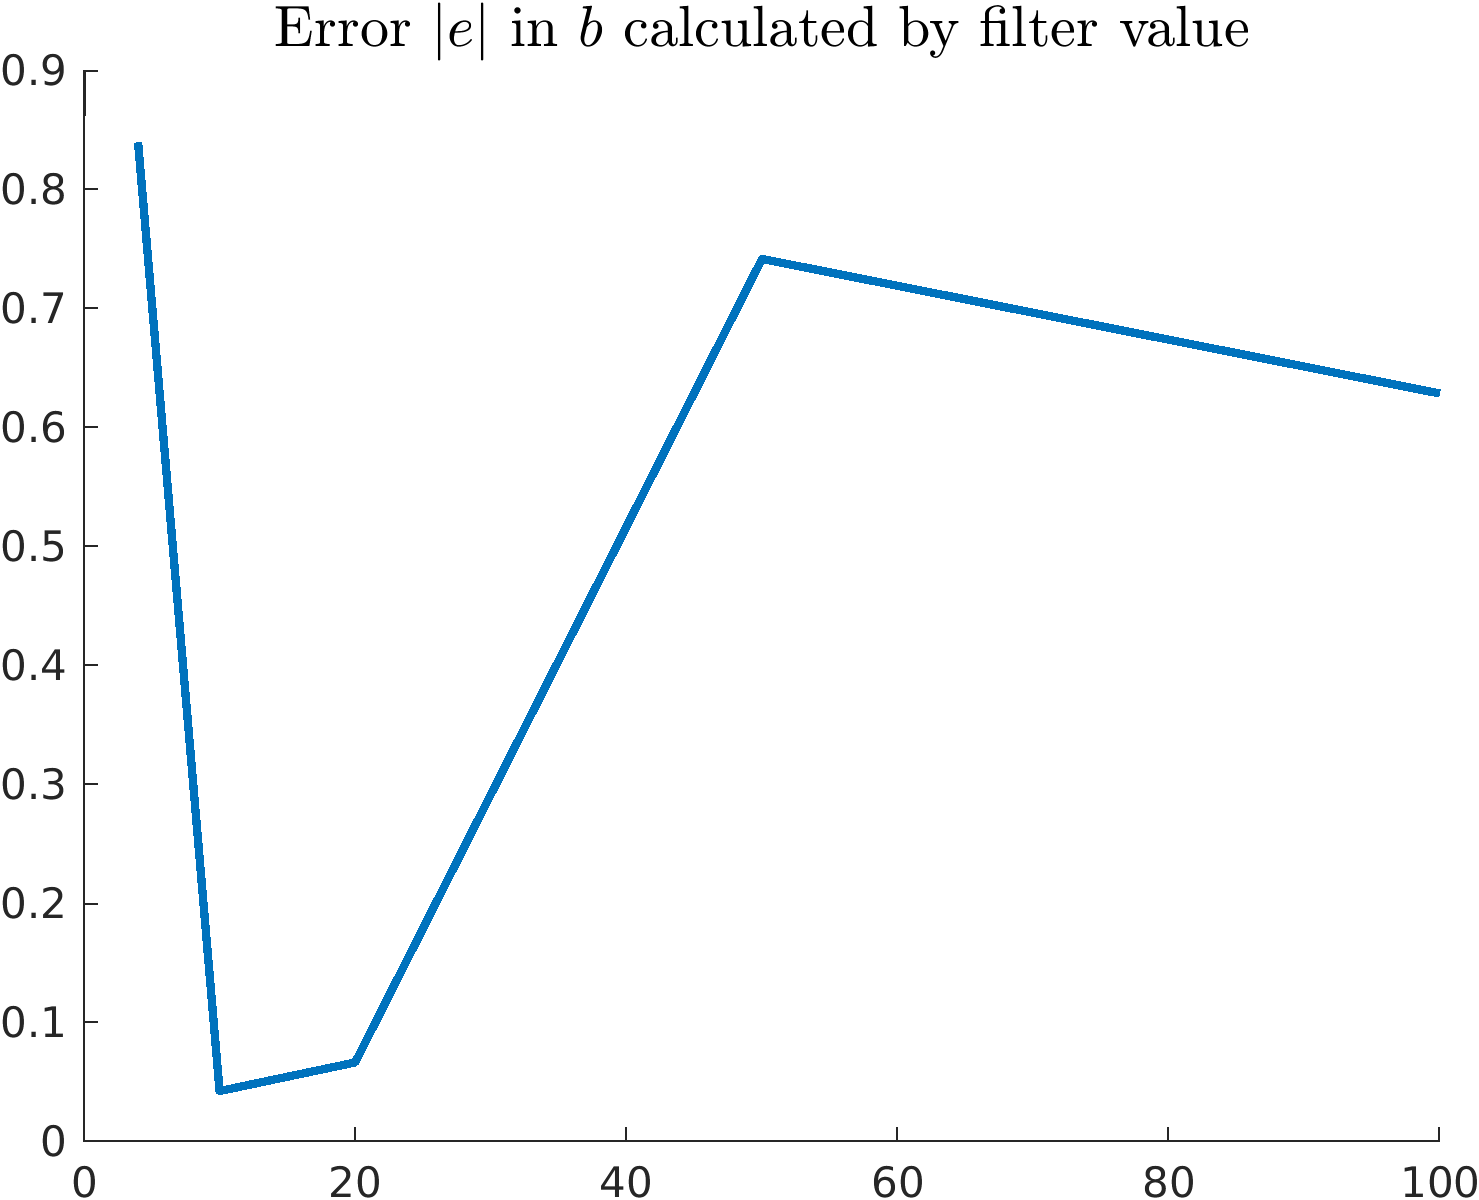
\includegraphics[width = \textwidth]{figures/filter_b_error.png}
        \caption{Error of b}
    \end{subfigure}
    \begin{subfigure}{0.325\textwidth}
        \centering
        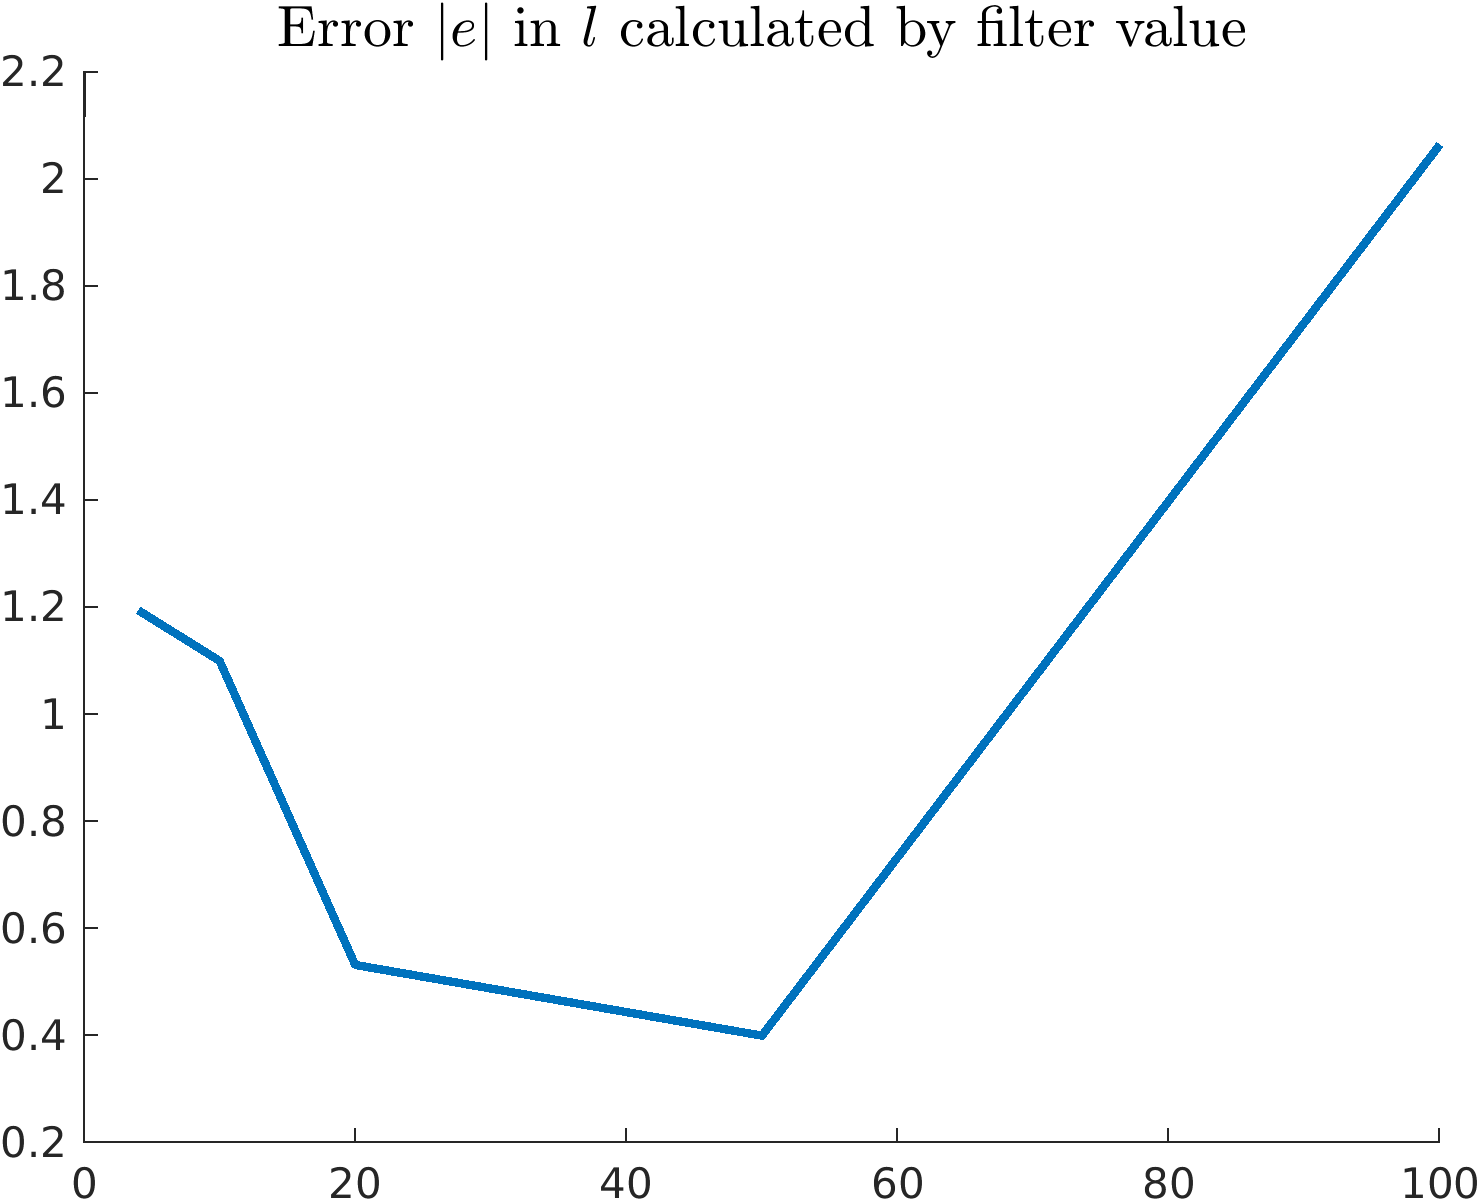
\includegraphics[width = \textwidth]{figures/filter_l_error.png}
        \caption{Error of l}
    \end{subfigure}
    \begin{subfigure}{0.325\textwidth}
        \centering
        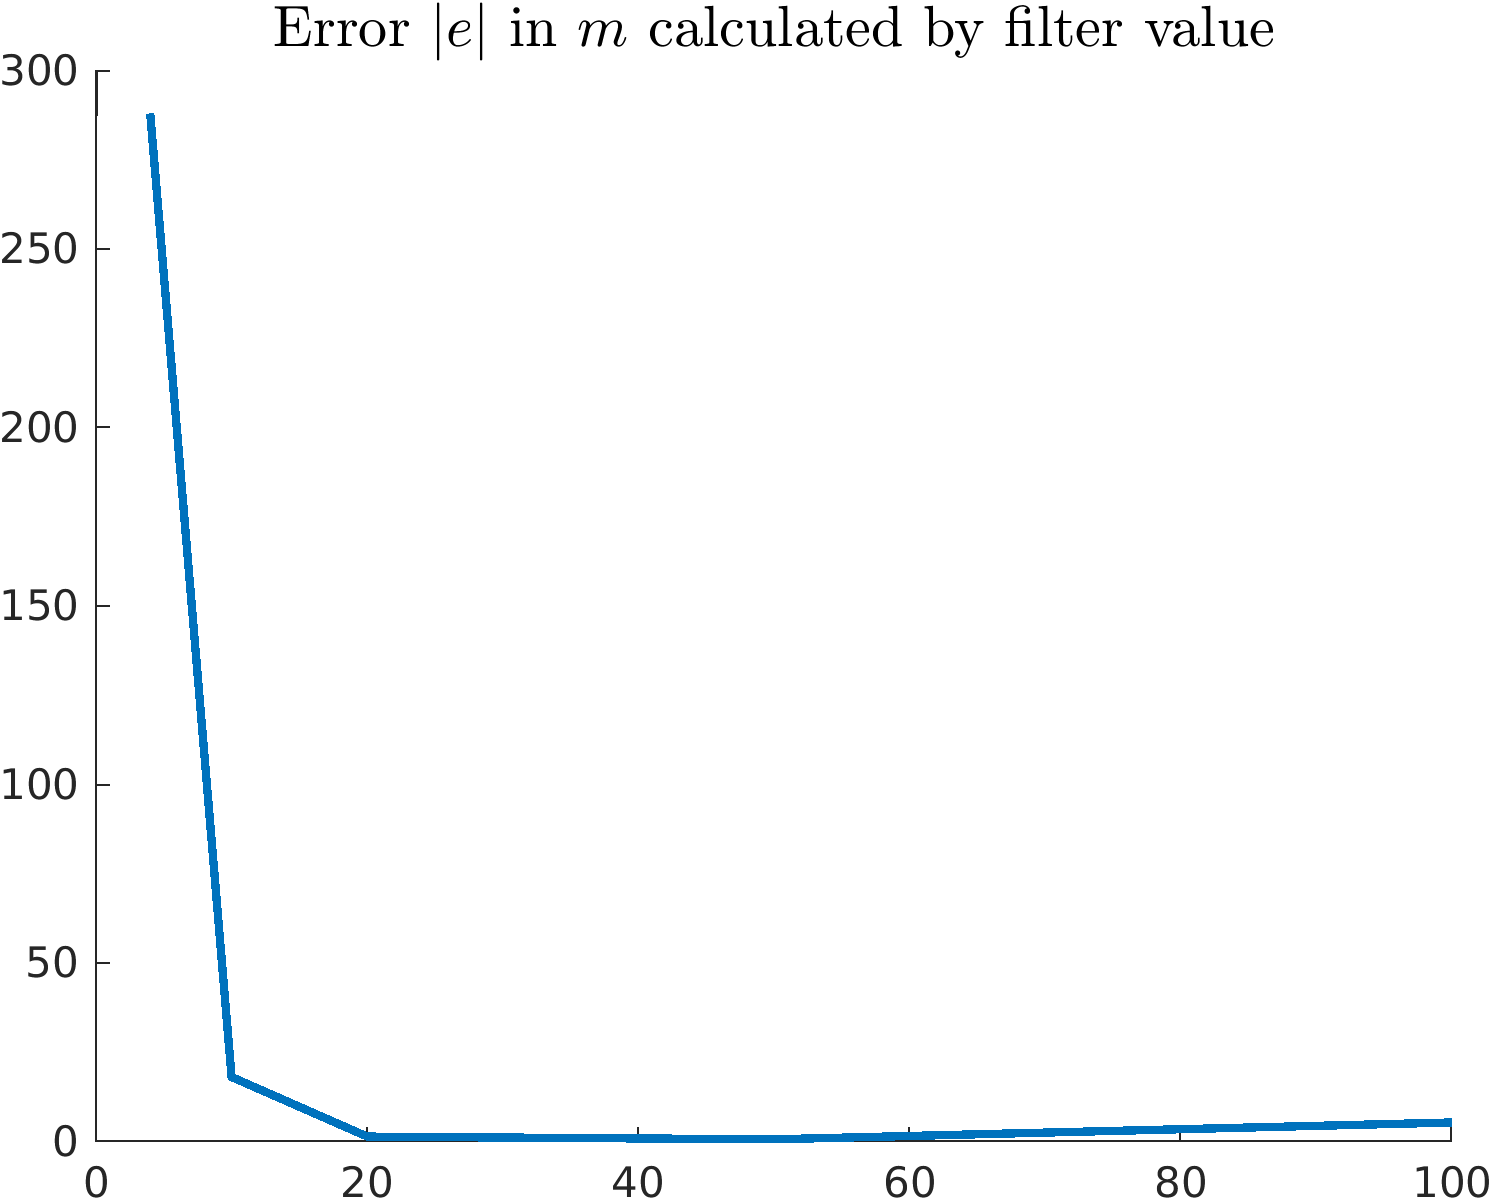
\includegraphics[width = \textwidth]{figures/filter_m_error.png}
        \caption{Error of m}
    \end{subfigure}
    \caption{$|e|$ error for $b$, $l$, and $m$ for a given moving filter mean with given $k$ values}
    \label{fig:b-3_results}
\end{figure}

The error when $k=4$ for the mass is so large that we provide the alternative figure dropping $k=4$:

\begin{figure}[H]
    \centering
    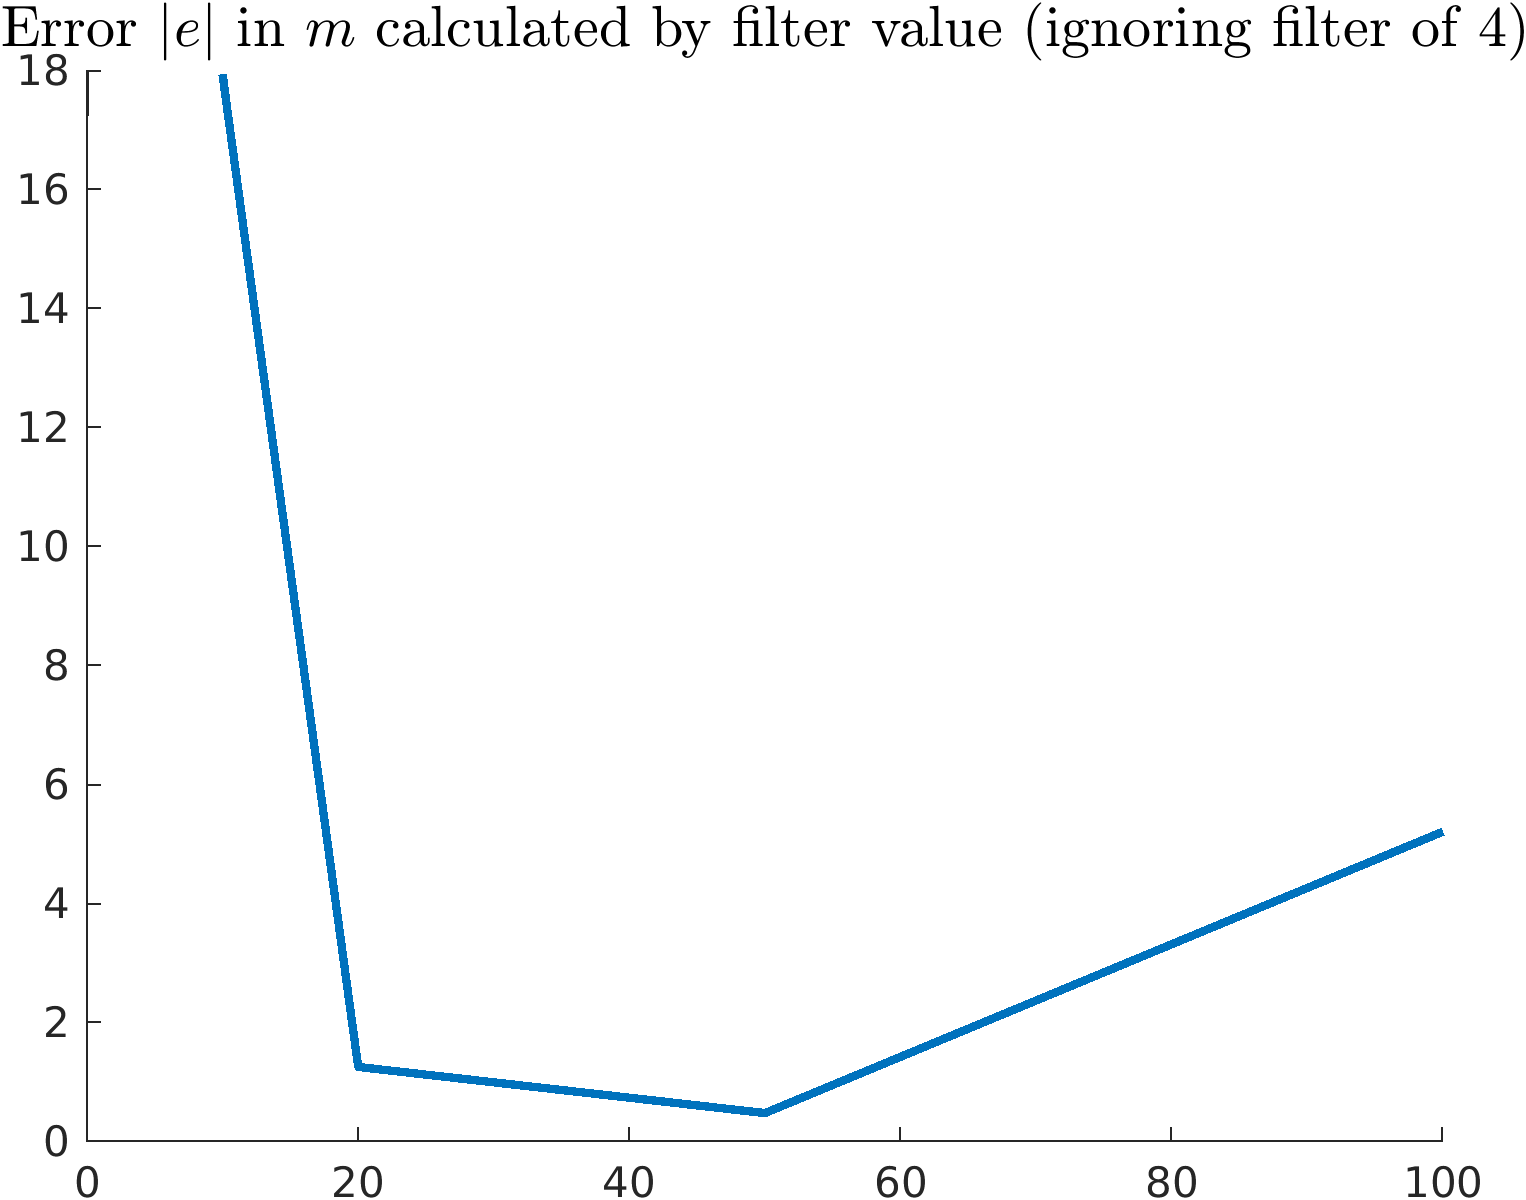
\includegraphics[width = 0.4\textwidth]{figures/filter_m_error_2.png}
    \caption{$|e_m|$ dropping $k=4$}
\end{figure}

Here we see that choosing the correct $k$ for the filter can cause large swings in accuracy of the calculated output of the parameters - it seems best to aim for some small percentage (but not too small) of moving average based on the dataset size. The amount of time between steps likely should be considered when doing this - a large enough $\Delta t$ between data reads would result in similar wild swings of calculated parameters.

Next, we looked at not using the Taylor Series approximation of each derivative but instead explored a directly observed derivative. Or, in other terms:

\begin{equation}
    \dot{q} = \frac{q_{i+1}-q_i}{\Delta t}
\end{equation}

\begin{equation}
    \ddot{q} = \frac{\dot{q}_{i+1}\dot{q}_i}{\Delta t}
\end{equation}

Note that we still performed the moving average filter on the $q$, $\dot{q}4$, and $\ddot{q}$ values before their usage to calculate its further derivative. We also performed the moving average filter on the $u(t)$ values. For each we used a $k=20$ and for $u(t)$ $k=10$, same as the original problem.

Our calculated values for $a$, $b$, $c$, $l$, and $m$, respecively, are:

\begin{equation}
    \begin{bmatrix}
        a \\
        b \\
        c \\
    \end{bmatrix} = \begin{bmatrix}
        3.858 \\
        0.914 \\
        27.723
    \end{bmatrix}
\end{equation}

...which leads to a $l=1.365$ and $m=2.070$. Our resulting errors are thus $e_b = 0.586$, $e_l = 0.165$, and $e_m = 0.230$. This is actually quite close, better than our original Taylor Series approximation method.

\end{document}